\section{Experimental results}\label{sec:expres}
%% We have implemented our above-described falsification algorithm using
%% the robustness evaluation function implemented in the Breach
%% toolbox~\cite{BreachCAV10}\footnote{We used the latest version
%% available in October 2016, on the
%% site \url{https://people.eecs.berkeley.edu/~donze/breach_page.html}}. In
%% our experiments, we first use two Simulink models having input and
%% output signals and test robustness of STL properties specified on the
%% output signals. These models have been used as benchmarks for
%% evaluating hybrid systems verification and validation techniques. In
%% addition, we also test our approach on an industrial system, which is
%% an air path controller for an automotive fuel cell (FC) application.

In our experiments, we compare the performance of a MATLAB
implementation of the combined metaheuristics algorithm with traditional falsification algorithms. Our implementation uses
the robustness evaluation function together with the following solvers CMA-ES, Simulated Annealing, and Global
Nelder-Mead algorithm implementations integrated in
Breach~\cite{DBLP:conf/cav/Donze10}. 
Our experiments were performed on a computer with 1.4GHz processor with 4GB RAM, running 
MATLAB R2015 64-bit version. 
In the following we first describe the models and the input and parameter settings of the benchmarks. Then we present the experimental results obtained using the new algorithm in comparison with the traditional search techniques used alone. Also, we compare it with a method combining
the CMA-ES and classification \cite{CAV2017}, where in each iteration the visited points are classified in order to identify promising regions.
%The grid used in this method is the same as the grid chosen to define the coverage.  %We will
%call this method as grid based random sampling, for the sake of
%reference during comparison.


\subsubsection*{{\em Automative Powertrain Control}.} \label{sec:PTC}
We consider a Simulink model of a closed-loop Automative Powertrain Control
subsystem (PTC). The model contains a representation of an internal combustion engine and an
embedded software controller for the air-to-fuel ratio within the
engine (see~\cite{Dreossi2015} for more details). The model has three input signals,
Pedal Angle, Engine Speed, and Sensor Offset.
The air-to-fuel (A/F) ratio, denoted by $\eta$, is an
output signal for which the following safety requirement: %$\phi = \G_{[5,10]}\lt(\eta<0.5\rt)$.
$\G_{[5,50]}( (\eta[t] < 0.05) \land ( \eta[t] > - 0.05 ))$. We consider an input range for
the Pedal Angle as $[0,40]$ and fix the Engine Speed and
Sensor Offset as $1000$ and $1$, respectively. We use  a piecewise constant
signal for the Pedal Angle input, where the signal is parameterized by $10$
uniformly spaced control points.  

%We allow $\theta$ to take any value in $[0,40]$, while we fix $w=1000$ and $h=1$. 

%\paragraph{Input signal settings.}%The time horizon is $50$s. %Thus, we have a $10$ dimensional search space $\cpset$.% to search for a counterexample of $\phi$.  
%\emph{\textbf {Algorithm setting.}}  For our algorithm, {\bf TODO}
%The global search time is $\Tglobalmax= $ seconds.  
%The cell partitioning $\omega$ consists of hypercubes of side length $\epsilon=4$. 
%% The other algorithms, i.e., CMA-ES, uniform random search and Global
%% Nelder-Mead in Breach and S-TaLiRo and run for a
%% maximum time of $5000$s.


\subsubsection*{{\em Automatic transmission.}} \label{sec:autotrans}
This benchmark model of an Automatic Transmission control
system appeared in~\cite{DBLP:conf/cpsweek/HoxhaAF14}\footnote{The model
and property description of this benchmark is available at \url{http://cps-vo.org/node/12116}}.  The system has
two inputs, called throttle and brake, respectively, and two
outputs, called the engine speed, denoted by $w$ (RPM), and the vehicle
speed, denoted $v$ (mph). The property states that if the engine speed stays below a value
$\overline{w}$, then the vehicle speed $v$ does not exceed a threshold
$\overline{v}$ within $10$ seconds.  We specify the values of $\overline{w}$ and
$\overline{v}$ to be $2520$ and $50$, respectively, which gives the
following STL property: $\phi=\neg ((\F_{[0,10]}v>50)\wedge(\G w\leq
2520) )$ \cite{DBLP:conf/cpsweek/HoxhaAF14}. We use piecewise constant input
signals for testing, where the throttle signal is parametrized by $7$
control points and the brake has $3$ control points. Thus, we have a
$10$ dimensional search space.
%% The specified range
%% in~\cite{FainekosARCH1415} for both the throttle and break inputs was
%% $[0,100]$.

%\paragraph{Input signal and parameter settings.}
%Initially, the vehicle is at rest, when $v=0$ and $w=0$.  For the
%input signals, we consider smaller ranges than specified
%in~\cite{DBLP:conf/cpsweek/HoxhaAF14}, which makes the property $\phi$ more
%robust.  The throttle signal is allowed to vary between
%$[35,100]$ and the brake is allowed to vary between $[0,40]$.  The
%time horizon is set to $30$ seconds.  


%\emph{\textbf{Algorithm setting}}.  {\bf TODO}



%\emph{\textbf{Results.}}  {\bf To describe}
%Our algorithm (classification guided
%global search with local search) successfully found a counterexample in
%less than $2000$ seconds for all randomly chosen seeds. As an indication of the 
%number of classification operations that occurred, the final number of separate rectangles
%constructed for while testing the first seed were 31.  In comparison,
%the CMA-ES found a falsifier for two seeds 5000 and 15000 within
%2000 seconds but failed to do so on the other seeds.  The other methods were
%not successful in finding a falsifier within the default stopping time
%of 3000 seconds.  For this example, S-TaLiRo became stuck around a local
%optimum without any significant reduction in robustness value.  The
%results are presented in Table~\ref{tab:results}.  We note that for
%any fixed seed for random sampling, these results are reproducible.


\subsubsection*{{\em Diesel model.}} \label{sec:diesel} 
The third examples is an industrial closed-loop Simulink model of a prototype airpath controller for a diesel engine. The model is large, with more than 3000 blocks, more than 20 lookup tables and function blocks containing customized Matlab functions and legacy code. Moreover, more than half of these lookup tables are high dimen- sional (greater than one dimension). For this case study, we choose a safety property specifying upper bounds on the overshoot of a particular signal. This is represented by the following STL formula:  $\phi = \G_{[5,10]} (Out1[t] < 41.1)$ where $Out1$ is an output signal. Compared to the previous work \cite{Dreossi2015}, the new algorithm allows falsifying a much larger bound. 


\subsubsection*{{\em Results.}} 
The results are presented in Table~\ref{tab:results} and Table~\ref{tab:SeedResults}.  We note that for
any fixed seed, that is the index for a sequence of random numbers in MATLAB for random sampling, these results are reproducible. 
As one can see from the tables, our combined metaheuristics algorithm successfully found a counterexample in
less than the time-out limit for all the considered benchmarks and almost for all the seeds. 
The other methods either were not successful in finding a falsifier within the time-out limit or 
took more computation time. Indeed the metaheuristics used alone, in particular Simulated Annealing 
and Global Nelder-Mead, got stuck around local optima for these examples.


\begin{table}[ht]
\caption{Experimental results on the benchmarks with seed 5000}
%\vspace{-0.5em}
%\vspace{-1.5em}
\label{tab:results}
\begin{center}
\begin{tabular}{|c|c|c|c|}
\hline
\multirow{1}{*}{Search method} & \multicolumn{3}{|c|}{Computation time (s)} \\
\hline
\cline{2-4}
 &  PTC & Aut. Trans & Diesel    \\
\hline
\cline{2-4}
 CMA-ES & T.O (5000)  & T.O. (2000)  &  413.252  \\
\hline
\cline{2-4}
 Simulated Annealing &  T.O. (2000) & T.O. (2000)  & TO (2000)     \\
\hline
\cline{2-4}
Global Nelder-Mead &  T.O. (2000) &  TO (2000)  &  TO (2000)    \\
\hline
\cline{2-4}
Pseudo-random & & & \\ 
sampling &  TO (5000)  &  T.O. (2000) & TO (2000)    \\
\hline
\cline{2-4}
Classification + & & & \\ 
CMA-ES  \cite{CAV2017} & 2891  & 2891  & 996    \\
\hline
\cline{2-4}
 Combined + & & & \\ 
 Metaheuristics & 1276.80 &  899.15 & 299.501   \\
\hline
\end{tabular}
\end{center}
\caption{Experimental results on the benchmarks with seed 5000. T.O.($T$): Exceeded indicated time out limit which is $T$ seconds.
Property for the PTC model $\phi = \G_{[5,50]}( (\eta[t] < 0.05) \land ( \eta[t] > - 0.05 ))$. Property for the Automatic Transmission model $\phi =  \G(w[t] < 2520) \land  \F_{[0,10]}(v[t] > 50)$. Property for the Diesel Engine model   $\phi = \G_{[5,10]} (Out1[t] < 41.1)$. 
%\emph{Seed}: Index for a sequence of random numbers in MATLAB. \emph{Solver}: Algorithm used for falsification. \emph{Computation time}: Amount of time (in seconds) until falsification or default stopping after the time limit in parentheses. Computation time is reported for a computer with 1.4GHz processor and 4GB RAM, running MATLAB R2015 64-bit version. \emph{Falsification}: Boolean variable indicating whether the algorithm could falsify the property.
}
%\vspace{-4mm}%Put here to reduce too much white space after your table 
\end{table}


\begin{table}[ht]
%\vspace{-0.5em}
%\vspace{-1.5em}
\label{tab:SeedResults}
\begin{center}
\begin{tabular}{|c|>{\centering\arraybackslash}p{2cm}|>{\centering\arraybackslash}p{1.5cm}|>{\centering\arraybackslash}p{2cm}|>{\centering\arraybackslash}p{1.5cm}|}
\hline
Seed &  \multicolumn{2}{|c|}{Computation time (s)} \\
\hline
\cline{1-1}
 &  Classification + CMA-ES \cite{CAV2017}  & Meta- heuristics  \\
\hline
\cline{1-2}
 0 &   996   &   991.41   \\
\hline
 5000 & 1382   &  899.15   \\
 \hline
10000 &  1720  &  966.87  \\
\hline
15000 &  1355  & 911.55  \\
\hline
\end{tabular}
\end{center}
\caption{Experiments with different seeds on the Automatic Transmission benchmark. Property $\phi =  \G(RPM[t] < 2520) \land  \F_{[0,10]}(speed[t] > 50)$.}
% \emph{Solver}: Algorithm used for falsification. \emph{Computation time}: Amount of time (in seconds) until falsification or default stopping after the time limit in parentheses. Computation time is reported for a computer with 1.4GHz processor and 4GB RAM, running MATLAB R2015 64-bit version. \emph{Falsification}: Boolean variable indicating whether the algorithm could falsify the property.}
%\vspace{-4mm}%Put here to reduce too much white space after your table 
\end{table}

\subsubsection*{$\Sigma \Delta$ modulator.}
 We illustrate the interest of timed pattern generation with a $\Sigma \Delta$ modulator which is an important component of $\Sigma \Delta$ analog-to-digital converters. Such converters have been widely used for analog signals of a large range of frequencies. Practical quantizers have a limited input and output ranges, which may lead them to saturation. We apply our methods of signal generation to test if a saturation can occur in a $\Sigma \Delta$ modulator. We use a behavioral model of a second-order modulator specified using Simulink\textsuperscript{\textregistered}, which takes into account most non-idealities \cite{Brigati99}, including sampling jitter, integrator noise, op-amp parameters (finite gain, finite bandwidth, slew-rate and saturation voltages). In terms of model complexity, this Simulink model is heterogeneous including embedded Matlab code and mixing discrete-time and continuous-time components, which goes beyond the applicability of the existing formal verification tools. Simplified discrete-time $\Sigma \Delta$ modulator model without non-idealities, for which it is possible to derive its dynamics equations and thus optimization can be formulated and solved using optimization \cite{DangDM04} and statistical model-checking \cite{ClarkeDL10}.
\begin{figure}[htbp]
\resizebox{0.85\textwidth}{!}{
\begin{tikzpicture}[->,>=stealth',shorten >=1pt,auto,node distance=2.1cm, initial text={}]
   \node [accepting,state] (q0)                      {$q_4$};
   \node[accepting,state]          (q1) [right of=q0,yshift=-0.8cm]         {$q_5$};
   \node[accepting,state]          (q2) [left of=q1,yshift=-0.8cm]         {$q_6$};
   \node[accepting,state]          (q3) [left of=q0,yshift=-0.8cm]         {$q_3$};
   \node [accepting,state] (q2bis)    [left of=q3]                  {$q_2$};   
   \node [accepting,state] (q1bis)    [left of=q2bis]                  {$q_1$};
   \node [initial,accepting,state] (q0bis) [left of=q1bis]                      {$q_0$};
   \path (q0) edge [bend left] 
   node {$\begin{array}{c}
         x_1\in (1,6)\\ x_1:=0
   \end{array}$} (q1);
   \path (q1) edge [bend left] 
   node {$\begin{array}{c}
         x_2\in (1,6)\\
        x_2:=0
   \end{array}$} (q2);
   \path (q2) edge [bend left] 
   node {$\begin{array}{c}
         x_3\in (1,6)\\ x_3:=0
   \end{array}$} (q3);
   \path (q3) edge [bend left]  
   node {$\begin{array}{c}
         x_4\in (1,6)\\
        x_4:=0
   \end{array}$} (q0);
   \path (q0bis) edge node [above] {$\begin{array}{c}x_1\in (0,6)\\ x_1:=0\end{array}$} (q1bis);
   \path (q1bis) edge node [above] {$\begin{array}{c}x_2\in (0,6)\\ x_2:=0\end{array}$} (q2bis);
   \path (q2bis) edge node [above] {$\begin{array}{c}x_3\in (0,6)\\ x_3:=0\end{array}$} (q3);
\end{tikzpicture}
}
%\begin{tikzpicture}[->,>=stealth',shorten >=1pt,auto,node distance=1.2cm, initial text={$c=0$}]
%   \node [initial,state,accepting] (q0)                      {$0$};
%      \path (q0) edge [loop above]  node [above]  {$\begin{array}{c} c'=2 c+\lfloor t \rfloor,
%      c'_0=\lfloor t \rfloor,\\ c'_{-1}=c_0, c'_{-2}=c_{-1}, c'_{-3}=c_{-2},\\
%      \textcolor{purple}{c_0+c_{-1}+c_{-2}+c_{-3} \in\{1,2\}}\end{array}$} (q0);
%\end{tikzpicture}
\caption{A timed automaton for the period constraint.}
 \label{fig:4.5clocks}
\end{figure}
%(see Fig.~\ref{fig:DeltaSigma}),
%\begin{figure}[!ht]
%  \centering
%  \includegraphics[width=0.9\textwidth]{figures/DSfig.pdf}
%  \caption{$\Sigma \Delta$ model with non-idealities \cite{Brigati99}.\label{fig:DeltaSigma}}
%\end{figure}%\vspace{-1cm}
~\\
The timed automaton in Figure \ref{fig:4.5clocks} specifies a class of quasi-periodic signals with uncertain period drifting duration that ranges between $1$ and $6$. The period duration can be scaled to consider the frequency range of interest. We discretise the signal value space and associate each transition label with a signal value range. The first transitions are used to model uncertainty in phase shift. The transitions should reflect some bounded variability condition. Then the signals are constructed by linear interpolation between the values of the time instants. The absence of saturation can be expressed as a simple STL property, which states that throughout the simulation duration, the absolute value of the output of the saturation block in the first integrator is always smaller than the saturation voltage value (which is $1.145$). We generate a set of $50$ timed words using uniform sampling \cite{BBBK16}. Indeed the automaton n Figure \ref{fig:4.5clocks} is compact and thus used for illustration; for pattern generation we use an automaton with more locations for more refined value intervals, and the signal period varies from $10$ to $16$. The scaling factor for the period is $6 \times 10^{-7}$. For the optimization part, we use Algorithm \ref{algoSolverCombination} for guided  combination of metaheuristics, with $30$ time instant parameters. This experiment allows observing that combining optimization with timed pattern generation allows us to falsify the absence of saturation after using $22$ generated timed patterns. For comparison purposes, we designed a custom strategy to encode the timed automata constraint: we created a domain with variable time instants, and for each signal generated, we compute the period drifting and check whether it lies in the given bounds. Over $100$ signals generated this way, we reject $37$ (see Figure~\ref{fig:reject}). We note that this type of encoding was doable for this example, but can be much more involved for more complex TA and lead to much higher rejection rate, rendering falsification without our approach infeasible. 
\begin{figure}[htbp]
  \centering
  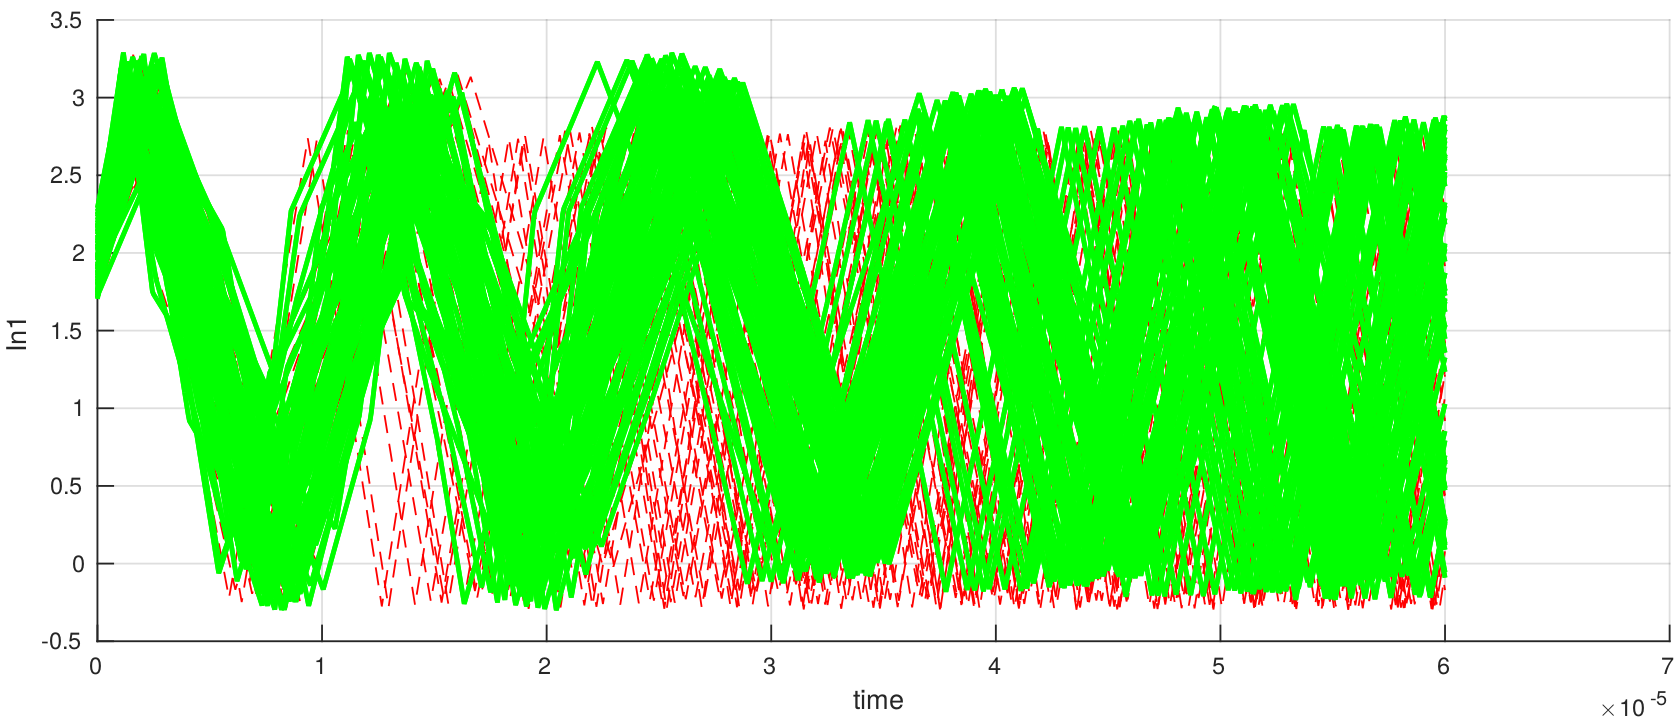
\includegraphics[width=\textwidth]{inputs_reject.png}
  \caption{The figure presents a set of $100$ signals generated with a custom method, of which 63 (green solid) satisfy the constraints of the timed automaton, and $37$ (red, dashed) do not.}
  \label{fig:reject}
 % \vspace{-3mm}
\end{figure}



%% \subsection{Benchmark experiment setup}

%% In our experiment, we try to compare the performance of a MATLAB implementation of our algorithm
%% with the following standard approaches: the uniform random sampling, CMA-ES,
%% Simulated annealing, Global Nelder Mead algorithm implementations (integrated in the same version of the tool 
%% Breach toolbox~\cite{BreachCAV10} that we used for our algorithm implementation), and the S-TaLiRo tool~\cite{TaliroLFS11} by setting Simulated Annealing as optimization algorithm\footnote{We used the latest version available in October 2016, on the site \url{https://sites.google.com/a/asu.edu/s-taliro/home}.}. Our
%% experiments were performed on a computer with 1.4GHz processor with 4GB
%% RAM, running MATLAB R2015 64-bit version. The settings of our algorithm as well as the other
%% falsification algorithm implementations are detailed below.


%% \subsubsection{Input signal specifications} 
%% \emph{Input signal range}.  We considered smaller ranges for
%% input signals than the ranges considered in the earlier
%% papers~\cite{Dreossi2015,FainekosARCH1415}, so that the properties become more robust and
%% consequently difficult to falsify.  F For the Automative Powertrain PTC example,
%% the Pedal Angle range is set as $[0,40]$ and Engine speed and Sensor
%% Offset signals are fixed as $1000$ and $1$, respectively.
%% %=======
%% %In our experiment, we try to compare the performance of our algorithm
%% %with standard approaches like uniform random sampling, CMAES,
%% %Simulated annealing, Global Nelder Mead and the an implementation
%% %distributed with the S-TaLiRo tool. Our
%% %experiments are performed on a computer with 1.4GHz processor with 4GB
%% %RAM.  The experimentes are implemented on MATLAB R2015 64-bit version.
%% %Our algorithm is implemented in the Breach toolbox~\textbf{CITE} for
%% %MATLAB-Simulink.  The setting of our algorithm as well as the other
%% %falsification algorithms is detailed below.
%% %
%% %
%% %\subsubsection{Input signal specifications} 
%% %\emph{Input signal range}.  We considered smaller ranges for input
%% %signals than the ranges considered in the earlier papers~\cite{todo},
%% %so that the properties become more robust and consequently difficult
%% %to falsify.  For the Automatic Transmission example, the throttle
%% %signal is allowed to vary between $[35,100]$ and the break is allowed
%% %to vary between $[0,40]$. For the Automative Powertrain PTC example,
%% %the Pedal Angle range is set as $[0,40]$ and Engine speed and Sensor
%% %Offset signals are fixed as $1000$ and $1$, respectively.
%% %>>>>>>> efa2003730ca38787c30f35819df6ca0f14cfe20

%% \emph{Finite parametrization of input signals.} We consider
%% piecewise constant input signals.  Furthermore, the allowed time
%% points of discontinuity for the piecewise constant signals are
%% uniformly spaced in the simulation time range of the signals.  For the
%% Automatic Transmission example, the throttle signal has $7$ control
%% points and the break signal has $3$ control points. So, we have
%% $m=7+3=10$ dimensional parameterized input signal space $\cpset$.  For the
%% Automative Powertrain Control example, we have $10$ control points,
%% thus, $\cpset$ is a $10$-dimensional space.


%% \subsubsection{Algorithm settings} 
%% \paragraph{Our algorithm setting}
%% \begin{itemize}
%% \item Threshold number of samples of hyperplane classification $K_c$ is
%% $70$ for the Automatic Transmission example and $100$ for the
%% Automative Powertrain Control example. For the Automatic Transmission
%% example, the influence of the break signal is not as much as that of the
%% throttle signal. Hence we considered a smaller threshold for
%% classification compared to the Automative Powertrain Control example.
%% %
%% \item Cell partitioning $\omega$ consists of hypercubes of side
%% length $\epsilon=4$ for both examples.
%% %
%% \item Global search time is $\Tglobalmax=500s$ for Automatic Transmission, while
%% $\Tglobalmax=2000s$ for the Automative Powertrain Control example.  The
%% Automative Powertrain example has a higher global search time because
%% the time of each function evaluation (simulation) is higher.
%% \item Local search settings. The CMA-ES implementation from
%% Breach-MATLAB toolbox was run for $4$ random number generating seeds: $0$,
%% $5000$, $10000$ and $15000$. The maximum time for the algorithm is
%% set to $2000$s for Automatic Transmission example and $5000$s for Automative Powertrain Control example.
%% \end{itemize}



%% \paragraph{S-TaLiRo setting.}  The Automatic transmission example is available in the distribution of
%% S-TaLiRo\footnote{The used distribution is available at~\url{sites.google.com/a/asu.edu/s-taliro/s-taliro/download}}.
%% For our experiment, we run the script provided in the distribution
%% with the following changes and specifications.  The range of throttle
%% input is reduced to $[35,100]$, while the original script specified
%% it as $[0,100]$.  The break input range is reduced to $[0,40]$, while
%% the original script has the range $[0,40]$.  We changed the class of
%% signals to piecewise constant.  Furthermore, we set the system to be a
%% black box, by setting the relevant S-TaLiRo options.  For the property
%% $\phi$, the script requires values for $\overline{\omega}$
%% and $\overline{v}$.  We specified them as $2520$ and $50$
%% respectively, according to the property we considered in the example.
%% The maximum number of tests (robustness evaluations) in the experiment
%% is set to $20000$.  The script runs the Simulated annealing algorithm
%% for falsification with the seed zero.  The default seed for random
%% number generation is set to $0$.


%% \paragraph{CMA-ES (in Breach) setting.}  The CMA-ES algorithm from Breach was run with the 
%% following setting.  We set the maximum time for the algorithm to $5000$s. The initialization vector is the mean of the
%% input-range.  We ran the algorithm with $4$ instances of seeds for
%% random number generation, i.e., seeds $0$, $5000$, $10000$ and $15000$.

%% \paragraph{Global-Nelder-Mead (in Breach) setting.} The
%% settings were specified in the default setup of Global-Nelder-Mead in
%% Breach.  The maximum time is set to $5000$ for the Automotive Powertrain and
%% $2000$ for the Automatic Transmission example.

%% \subsection{Benchmark results}  

%% The experimental results for the two benchmarks are reported in Table \ref{tab:results}.


%% For the Automatic Transmission example, just the global search phase
%% of our algorithm, i.e., without the CMA-ES local search, successfully
%% found a falsifier within $1000$s. In comparison, the CMA-ES algorithm
%% could not falsify within $2000$s for any of these seeds.  The uniform
%% random sampling procedure found a falsifier for only the
%% seed $15000$, but failed to find a falsifier within 2000s for the rest
%% seeds $0$, $5000$, $10000$, and $20000$.  Also, the Global Nelder Mead and
%% Simulated Annealing could not falsify within $2000$s and S-TaLiRo could
%% not falsify within $3000$s.

%% For the Automative Powertrain Control example, our algorithm successfully found
%% a falsifier within $3000$s for all the seeds.  This involved running
%% the global search phase for $2000$s followed by the CMA-ES local search
%% (until falsification).  However, the CMA-ES search alone, without
%% initialization guidance from hyperplane classification, could not
%% falsify within $5000$s for any of the above seeds.  The uniform random
%% sampling algorithm found a falsifier only for the seeds $10000$ and
%% $15000$, but failed to find falsifier within $5000$s for the rest seeds
%% $0,5000$ and $20000$.  The Global Nelder Mead and Simulated annealing
%% also could not falsify within $5000$s.


%\vspace{-1em}
%\subsection{Industrial example} 
%\input{FCexample.tex}
